\documentclass[11pt,a4paper]{article}
%--------------------------------------------------
%Packages bases
\usepackage{lmodern}
\usepackage[spanish]{babel}
\usepackage[utf8]{inputenc}
\usepackage{array}
\usepackage{ifthen}
\usepackage{transparent}
\usepackage{eso-pic}
\usepackage{multirow}
\usepackage{afterpage}
\usepackage{amsfonts}
\usepackage{amssymb}
\usepackage{amsthm}
\usepackage{float}
\usepackage{ifthen}
\usepackage{framed}
\usepackage{xspace}
\usepackage{multicol}
\usepackage{enumitem}
\usepackage{color}
\usepackage{titlesec}
\usepackage{ifthen}


%----------------------------------------
%design
\usepackage{amsmath,tikz}
\usepackage{verbatim}
\usetikzlibrary{shapes.geometric}
\usetikzlibrary{arrows}

%----------------------------------------
%color
\usepackage{transparent}
\usepackage{colortbl}
\definecolor{darkred}{rgb}{.7,0.03,0.22}
\definecolor{red_tab}{rgb}{0.96,0.88,0.86}
\definecolor{darkblue}{HTML}{0000CC}
\definecolor{vdarkblue}{HTML}{000066}
\definecolor{texte}{HTML}{660099}
\definecolor{comt}{HTML}{009933}
%-----------------------------------------


%------------------------------------------
%counters
\newcounter{step}
\newcounter{substep}
\setcounter{step}{0}
\setcounter{substep}{0}
%------------------------------------------

\usepackage{tabularx}
\usepackage{makecell}


\newcolumntype{R}[1]{>{\raggedleft\arraybackslash }p{#1}}
\newcolumntype{L}[1]{>{\raggedright\arraybackslash }p{#1}}
\newcolumntype{C}[1]{>{\centering\arraybackslash }p{#1}}

\usepackage{wasysym}


\usepackage{ifluatex}
\ifluatex
\usepackage{fontspec}
\usepackage{polyglossia}
\setdefaultlanguage{french}
\else
\usepackage[utf8]{inputenc}
\usepackage[T1]{fontenc}
\usepackage{babel}


%-----------------------------------------
%format page
\usepackage[a4paper,left=2cm,right=1cm,top=0.5cm,bottom=1cm,headheight=0cm, headsep=0cm, footskip=0cm,includefoot,includehead]{geometry}

%----------------------------------------
%footnote and header number
\usepackage{fancyhdr}
\usepackage[pages=all]{background}
\pagestyle{fancy}
\renewcommand{\headrulewidth}{0pt}
\fancyhf {} % clear all headers and footers

% Header is used to include the page background
\backgroundsetup{
scale=1,
color=black,
opacity=1,
angle=0,
contents={%
  
\includegraphics[width=\paperwidth,height=\paperheight]{images/paper.jpg}
  }%
}

%-----------------------------------------
%Hyperlink
\usepackage[colorlinks, bookmarks, linkcolor=black, citecolor=black, urlcolor=blue]{hyperref}

%-----------------------------------------
%Set Monospace font
% \usepackage{everysel}
%     \renewcommand*\familydefault{\ttdefault}
%     \EverySelectfont{%
%     \fontdimen2\font=0.4em  % interword space
%     \fontdimen3\font=0.2em  % interword stretch
%     \fontdimen4\font=0.1em  % interword shrink
%     \fontdimen7\font=0.1em  % extra space
%     \hyphenchar\font=`\-    % to allow hyphenation
% }
%-----------------------------------------
%Configurations
\newcommand{\Style}[1]{
\ifthenelse{#1=1}{\makeatletter
\newcommand{\PrepTime}[1]{\def\@PrepTime{#1\xspace}
\def\PrepTimeb{#1}}
\newcommand{\CookingTime}[1]{\def\@CookingTime{#1\xspace}}
\newcommand{\background}[1]{%
\AddToShipoutPictureBG{\AtPageLowerLeft{\transparent{0.1}\includegraphics[width=\paperwidth,height=\paperheight]{#1}}}
}
\newcommand{\CookingTempe}[1]{%
\ifnum0=#1\relax
   \def\@CookingTempe{} 
\else
  \def\@CookingTempe{-- #1$^{\circ}$} 
\fi
}

\newcommand{\TypeCooking}[1]{\def\@TypeCooking{#1}}
\newcommand{\NPerson}[1]{\def\@NbPerson{#1\xspace}}
\newcommand{\Image}[2]{\def\@ImageDim{#1} \def\@ImagePath{#2}}
\def\maketitle{%

\vspace*{0.05cm}
\begin{center}
{\Huge \@title}
\end{center}
}

\newenvironment{ingredient}
  {\noindent\begingroup\edef\x{\endgroup\noexpand}\x
  \maketitle
  
  \begin{footnotesize}\noindent\setlength\arrayrulewidth{2pt}\begin{tabular}{|L{0.62\linewidth}|L{0.33\linewidth}|}\hline\vspace{-0.21cm}\underline{\textbf{{\normalsize Ingredients (\@NbPerson persons):}}} &\\
  \begin{minipage}{\linewidth}
  \vspace{0.2cm}
  }
  {\vspace{-0.2cm}
  \end{minipage}& \vspace{-1.8cm}Preparation time: \begin{tikzpicture}
  \pgfmathsetmacro{\timeor}{\PrepTimeb}
  \ifthenelse{\timeor>60}{
  \pgfmathsetmacro{\timeorb}{90-(\PrepTimeb-60)/60*360}
  \fill[orange] (0,0.55) arc(90:-270:0.55)      -- ++(-270:-0.55)
  arc(-270:0:0)    -- cycle;
  \fill[red] (0,0.55) arc(90:\timeorb:0.55)      -- ++(\timeorb:-0.55)
  arc(\timeorb:0:0)    -- cycle;
  }{
  \pgfmathsetmacro{\timeorb}{90-(\PrepTimeb)/60*360}
  \fill[green] (0,0.55) arc(90:\timeorb:0.55)      -- ++(\timeorb:-0.55)
  arc(\timeorb:0:0)    -- cycle;
  }
  \node[fill=white,inner sep=0pt] at (0,0) {{\tiny \PrepTimeb~min}};
  \fill[black!50,even odd rule] (0,0) circle(0.65) circle(0.6);
  \fill[black!50,even odd rule] (0,0.5) circle(0.05);
  \fill[black!50,even odd rule] (0.5,0) circle(0.05);
  \fill[black!50,even odd rule] (0,-0.5) circle(0.05);
  \fill[black!50,even odd rule] (-0.5,0) circle(0.05);
  \end{tikzpicture} \par
  \vspace{0.2cm} Cooking: \@CookingTime min \@CookingTempe

  
   \par \vspace{0.2cm} Cooking Type: \@TypeCooking \\\hline\end{tabular}\vspace{0.5cm} \end{footnotesize}}


\newenvironment{main}
  {\begin{multicols}{2}
  \begin{itemize}[label=$$]
  }
  {\end{itemize}\end{multicols}}
  
\newenvironment{subingredient}[1]
{\vspace{-0.3cm}\hspace{0.5cm}\underline{#1:}
\vspace{-0.3cm}\begin{multicols}{2}
\begin{itemize}[label=$$]
}
{\end{itemize}\end{multicols}}


\newenvironment{recipe}
{
}
{}
\makeatother

%-----------------------------------------
%New environments

\newenvironment{notes}
{\vfill\def\FrameCommand{\fboxsep=\FrameSep\fbox}%
\MakeFramed {\advance\hsize-\width \FrameRestore}
\noindent\underline{\textbf{Notes and tips:}}%

\vspace{0.25cm}
\noindent\hspace{-0.15cm}}
{\vspace{2.5cm}\endMakeFramed}
  
  
\newcommand{\step}[1]{\ifthenelse{\value{step}=0}{\noindent{\large \underline{\textbf{Preparation:}}}\vspace{0.3cm}

}{}
\noindent\stepcounter{step}\setcounter{substep}{0}\the\value{step}. #1\vspace{0.3cm}

} 

\newcommand{\substep}[2][1]{\ifthenelse{\value{substep}=0}{\noindent\stepcounter{step}\the\value{step}. \underline{\textbf{#1:}}\vspace{0.3cm}

}{}
\hspace{0.3cm}\begin{minipage}{0.948\textwidth}
\noindent\stepcounter{substep}\roman{substep}. #2\vspace{0.5cm}
\end{minipage}

}   }{}
\ifthenelse{#1=2}{\makeatletter
\newcommand{\PrepTime}[1]{\def\@PrepTime{#1\xspace}
\def\PrepTimeb{#1}}
\newcommand{\CookingTime}[1]{\def\@CookingTime{#1\xspace}}
\newcommand{\background}[1]{%
\AddToShipoutPictureBG{\AtPageLowerLeft{\transparent{0.1}\includegraphics[width=\paperwidth,height=\paperheight]{#1}}}
}
\newcommand{\CookingTempe}[1]{%
\ifnum0=#1\relax
   \def\@CookingTempe{} 
\else
  \def\@CookingTempe{-- #1$^{\circ}$} 
\fi
}

\newcommand{\TypeCooking}[1]{\def\@TypeCooking{#1}}
\newcommand{\NPerson}[1]{\def\@NbPerson{#1\xspace}}
\newcommand{\Image}[2]{\def\@ImageDim{#1} \def\@ImagePath{#2}}
\def\maketitle{%

\vspace*{0.05cm}
\begin{center}
{\Huge \@title}
\end{center}
}

\newenvironment{ingredient}
  {\noindent\begingroup\edef\x{\endgroup\noexpand}\x
  \maketitle
  
  \begin{footnotesize}\noindent\setlength\arrayrulewidth{2pt}\begin{tabular}{|L{0.62\linewidth}|L{0.33\linewidth}|}\hline\vspace{-0.21cm}\underline{\textbf{{\normalsize Ingredientes (\@NbPerson personas):}}} &\\
  \begin{minipage}{\linewidth}
  \vspace{0.2cm}
  }
  {\vspace{-0.2cm}
  \end{minipage}& \vspace{-1.8cm}Tiempo de preparación: \begin{tikzpicture}
  \pgfmathsetmacro{\timeor}{\PrepTimeb}
  \ifthenelse{\timeor>60}{
  \pgfmathsetmacro{\timeorb}{90-(\PrepTimeb-60)/60*360}
  \fill[orange] (0,0.55) arc(90:-270:0.55)      -- ++(-270:-0.55)
  arc(-270:0:0)    -- cycle;
  \fill[red] (0,0.55) arc(90:\timeorb:0.55)      -- ++(\timeorb:-0.55)
  arc(\timeorb:0:0)    -- cycle;
  }{
  \pgfmathsetmacro{\timeorb}{90-(\PrepTimeb)/60*360}
  \fill[green] (0,0.55) arc(90:\timeorb:0.55)      -- ++(\timeorb:-0.55)
  arc(\timeorb:0:0)    -- cycle;
  }
  \node[fill=white,inner sep=0pt] at (0,0) {{\tiny \PrepTimeb~min}};
  \fill[black!50,even odd rule] (0,0) circle(0.65) circle(0.6);
  \fill[black!50,even odd rule] (0,0.5) circle(0.05);
  \fill[black!50,even odd rule] (0.5,0) circle(0.05);
  \fill[black!50,even odd rule] (0,-0.5) circle(0.05);
  \fill[black!50,even odd rule] (-0.5,0) circle(0.05);
  \end{tikzpicture} \par
  \vspace{0.2cm} Cocción: \@CookingTime min \@CookingTempe

   \par \vspace{0.2cm} Tipo de cocción: \@TypeCooking \\\hline\end{tabular}\vspace{0.5cm} \end{footnotesize}}


\newenvironment{main}
  {\begin{multicols}{2}
  \begin{itemize}[label=$$]
  }
  {\end{itemize}\end{multicols}}
  
\newenvironment{subingredient}[1]
{\vspace{-0.3cm}\hspace{0.5cm}\underline{#1:}
\vspace{-0.3cm}\begin{multicols}{2}
\begin{itemize}[label=$$]
}
{\end{itemize}\end{multicols}}


\newenvironment{recipe}
{
}
{}
\makeatother

%-----------------------------------------
%New environments

\newenvironment{notes}
{\vfill\def\FrameCommand{\fboxsep=\FrameSep\fbox}%
\MakeFramed {\advance\hsize-\width \FrameRestore}
\noindent\underline{\textbf{Notas y tips:}}%

\vspace{0.25cm}
\noindent\hspace{-0.15cm}}
{\vspace{1cm}\endMakeFramed}
  
  
\newcommand{\step}[1]{\ifthenelse{\value{step}=0}{\noindent{\large \underline{\textbf{Preparación:}}}\vspace{0.3cm}

}{}
\noindent\stepcounter{step}\setcounter{substep}{0}\the\value{step}. #1\vspace{0.3cm}

} 

\newcommand{\substep}[2][1]{\ifthenelse{\value{substep}=0}{\noindent\stepcounter{step}\the\value{step}. \underline{\textbf{#1:}}\vspace{0.3cm}

}{}
\hspace{0.3cm}\begin{minipage}{0.948\textwidth}
\noindent\stepcounter{substep}\roman{substep}. #2\vspace{0.5cm}
\end{minipage}

}   }{}}



\newcommand{\grado}{Grado en ingeniería en electrónica, robótica y mecatrónica}
\newcommand{\asignatura}{Sistemas Electrónicos}
\newcommand{\actividad}{Tareas puntuables}
\newcommand{\titulo}{RAM-based Shift Register}
\newcommand{\subtitulo}{Tarea \# 3}
\newcommand{\descripcion}{Análisis de un registro de desplazamiento basado en la RAM.}
\newcommand{\foto}{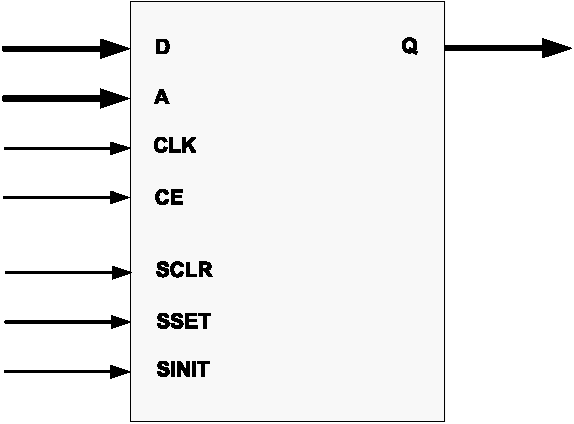
\includegraphics[scale=0.75]{images/registro_de_desplazamiento.pdf}}
\newcommand{\curso}{2021-2022}
\newcommand{\autor}{Jorge Benavides Macías \\ 05306948-C}
\begin{document}
% %%%%%%%%%%%%%%%%%%%%%%%%%%%%%%%%%%%%%%%%%%%%%%%%%%%%%%%%%%%%%%%%%%%%%%%%
% Plantilla TFG/TFM
% Escuela Politécnica Superior de la Universidad de Alicante
% Realizado por: Jose Manuel Requena Plens
% Contacto: info@jmrplens.com / Telegram:@jmrplens
%%%%%%%%%%%%%%%%%%%%%%%%%%%%%%%%%%%%%%%%%%%%%%%%%%%%%%%%%%%%%%%%%%%%%%%%


\begin{titlepage}

% Márgenes de esta pagina modificados
\newgeometry{ignoreall,top=2cm,bottom=2cm}
\setlength{\centeroffset}{-0.5\oddsidemargin}
\addtolength{\centeroffset}{0.5\evensidemargin}
\thispagestyle{empty}

\AddToShipoutPictureBG*{%
\begin{tikzpicture}[overlay,remember picture]
\draw[line width=10pt]
    ($ (current page.north west) + (2cm,-2cm) $)
    rectangle
    ($ (current page.south east) + (-2cm,2cm) $);
\draw[line width=1.5pt]
    ($ (current page.north west) + (2.2cm,-2.2cm) $)
    rectangle
    ($ (current page.south east) + (-2.2cm,2.2cm) $);
\end{tikzpicture}
}

\FuenteTitulo
\centering
\vspace*{5em}
{\fontsize{30pt}{0pt}\selectfont \seguridadx}
\vfill
{\fontsize{25pt}{0pt}\selectfont \identificadorx}
\vfill
{\fontsize{25pt}{0pt}\selectfont \organizacionx}
\vfill
{\fontsize{25pt}{0pt}\selectfont \ul\titulox}
\vfill
% {\fontsize{20pt}{0pt}\selectfont \subtitulox}
% \vfill
{\fontsize{20pt}{0pt}\selectfont \autorx}

\vspace{1em}
{\fontsize{15pt}{0pt}\selectfont \asociacionx}
\vfill
{\fontsize{10pt}{0pt}\selectfont \fechax}
\vfill
{\fontsize{25pt}{0pt}\selectfont \tipox}
\vfill
{\fontsize{30pt}{0pt}\selectfont \seguridadx}
\vspace*{5em}
\vfill

% \def\FuenteTamano{50pt}
% % Titulo y subtitulo
% \vspace*{5em}
% \def\FuenteTamano{30pt}
% {\FuenteTitulo\fontsize{\FuenteTamano}{0pt}\selectfont\color{black} \seguridadx}
% \vfill
% \def\FuenteTamano{25pt}
% {\FuenteTitulo\fontsize{\FuenteTamano}{0pt}\selectfont\color{black} \identificadorx}
% \vfill
% {\FuentePortada \fontsize{\TamTrabajo}{35pt}\selectfont\color{black}\organizacionx}
% \vfill
% {\raggedright{\FuenteTitulo\fontsize{\FuenteTamano}{35pt}\selectfont\color{black} \titulox}}
% \vfill
% % {\raggedright{\FuenteTitulo\fontsize{\FuenteTamano}{110pt}\selectfont\color{black} \subtitulox }}
% % \vfill
% {\FuentePortada \fontsize{\TamTrabajo}{25pt}\selectfont\color{black} \autorx}
% \vfill
% {\FuentePortada \fontsize{\TamOtros}{30pt}\selectfont\color{black}\fechax}
% \vfill
% {\FuentePortada \fontsize{\TamTrabajo}{30pt}\selectfont\color{black}\tipox}
% \vfill
% \def\FuenteTamano{30pt}
% {\FuenteTitulo\fontsize{\FuenteTamano}{0pt}\selectfont\color{black} \seguridadx}
% \vspace{2cm}
% \vfill
\end{titlepage}

% A partir de aquí aplica los márgenes establecidos en configuracioninicial.tex
\restoregeometry

\begin{itemize}
    \item Configuración del CORE GENERATOR.
    
    \begin{figure}[H]
        \centering
        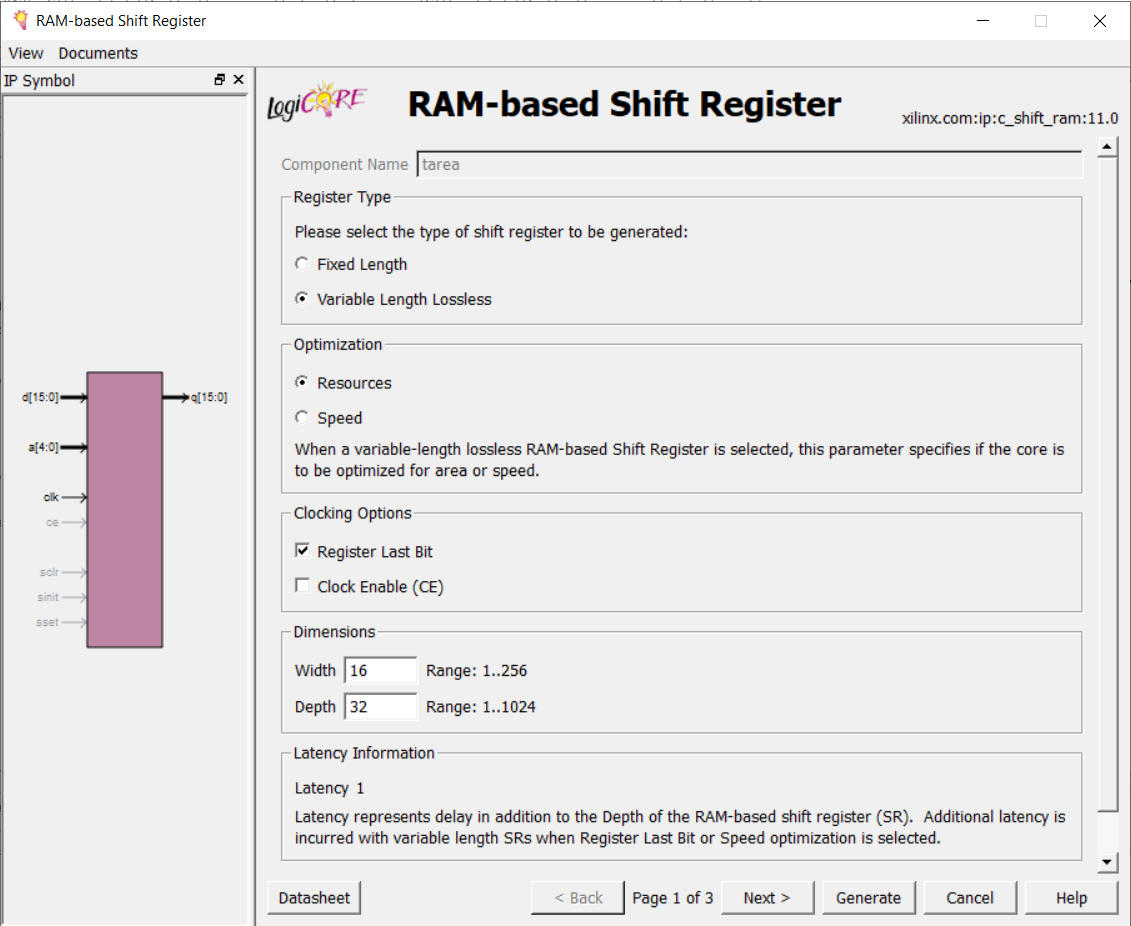
\includegraphics[scale=0.5]{images/core_1.png}
        \caption{Ventana de configuración. Página 1 de 3.}
    \end{figure}
    
    \begin{figure}[H]
        \centering
        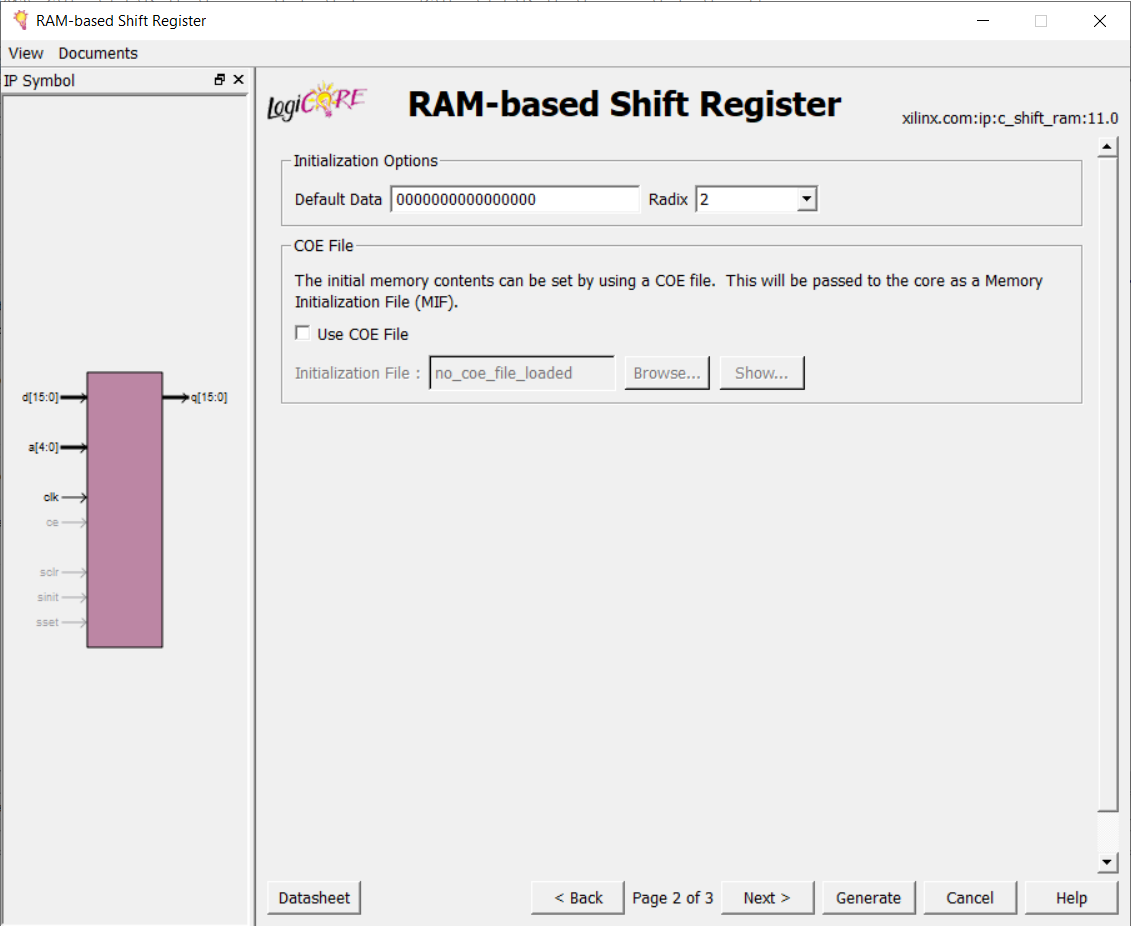
\includegraphics[scale=0.5]{images/core_2.png}
        \caption{Ventana de configuración. Página 2 de 3.}
    \end{figure}
    
    \begin{figure}[H]
        \centering
        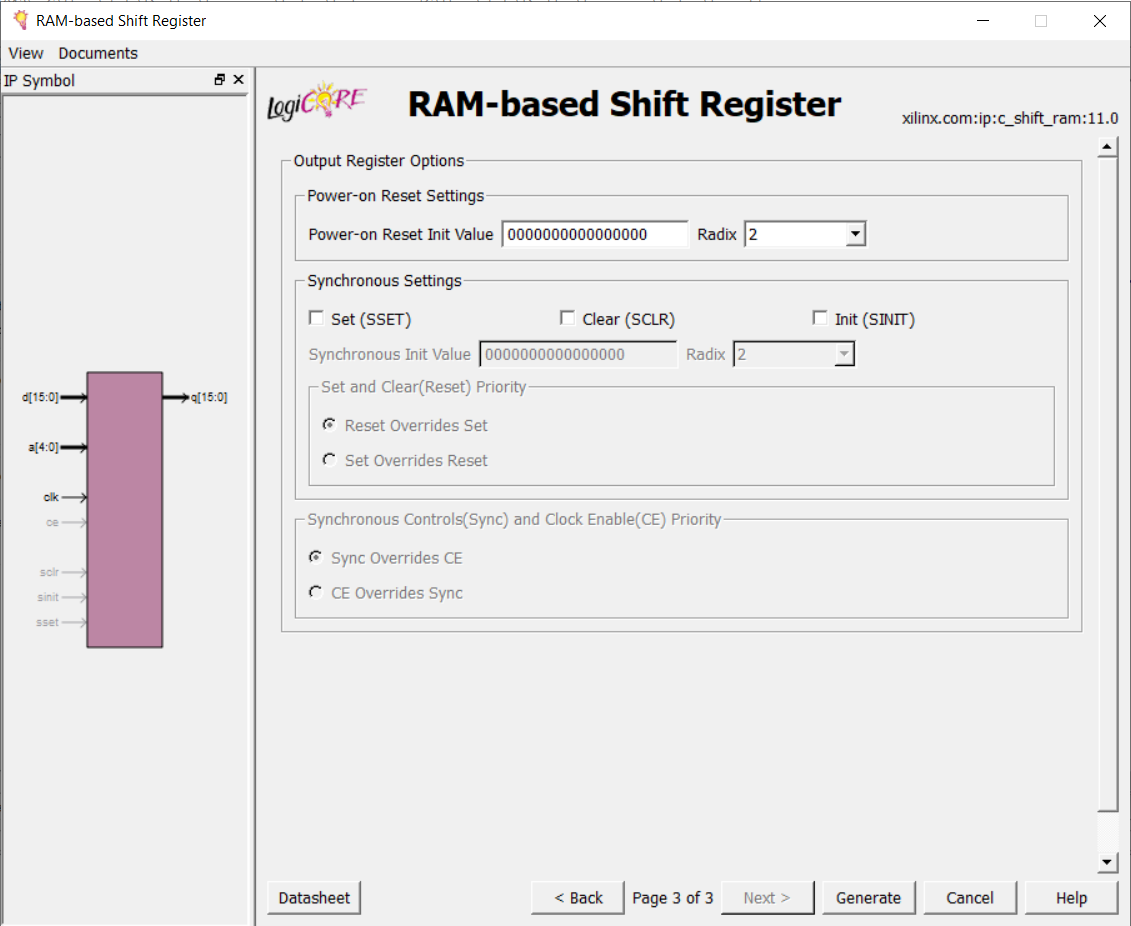
\includegraphics[scale=0.5]{images/core_3.png}
        \caption{Ventana de configuración. Página 3 de 3.}
    \end{figure}
    
    \item Script de simulación.
    
\begin{minted}[frame=lines,framesep=2mm,baselinestretch=1.2,bgcolor=LightGray,fontsize=\footnotesize,linenos]
{vhdl}
-- Vhdl test bench created from schematic C:\Users\rhylo\Desktop\tarea_seee\testing\top.sch 
-- Thu Dec 19 17:09:33 2021
-- Notes: 
-- 1) This testbench template has been automatically generated using types
-- std_logic and std_logic_vector for the ports of the unit under test.
-- Xilinx recommends that these types always be used for the top-level
-- I/O of a design in order to guarantee that the testbench will bind
-- correctly to the timing (post-route) simulation model.
-- 2) To use this template as your testbench, change the filename to any
-- name of your choice with the extension .vhd, and use the "Source->Add"
-- menu in Project Navigator to import the testbench. Then
-- edit the user defined section below, adding code to generate the 
-- stimulus for your design.
--
LIBRARY ieee;
USE ieee.std_logic_1164.ALL;
USE ieee.numeric_std.ALL;
LIBRARY UNISIM;
USE UNISIM.Vcomponents.ALL;
ENTITY top_top_sch_tb IS
END top_top_sch_tb;
ARCHITECTURE behavioral OF top_top_sch_tb IS 

   COMPONENT top
   PORT( d	:	IN	STD_LOGIC_VECTOR (15 DOWNTO 0); 
          a	:	IN	STD_LOGIC_VECTOR (4 DOWNTO 0); 
          ck	:	IN	STD_LOGIC; 
          q	:	OUT	STD_LOGIC_VECTOR (15 DOWNTO 0));
   END COMPONENT;

   SIGNAL d	:	STD_LOGIC_VECTOR (15 DOWNTO 0);
   SIGNAL a	:	STD_LOGIC_VECTOR (4 DOWNTO 0);
   SIGNAL ck	:	STD_LOGIC;
   SIGNAL q	:	STD_LOGIC_VECTOR (15 DOWNTO 0);

BEGIN

   UUT: top PORT MAP(
		d => d, 
		a => a, 
		ck => ck, 
		q => q
   );

-- *** Test Bench - User Defined Section ***
CK_process :process
	begin
		CLOCK_LOOP : LOOP
		ck <= transport '0';
		WAIT FOR 4 ns;
		ck <= transport '1';
		WAIT FOR 5 ns;
		ck <= transport '0';
		WAIT FOR 1 ns;
		END LOOP CLOCK_LOOP;
  end process; 

   tb : PROCESS
   BEGIN
		d <= transport "0000000011111111";
		a <= transport "00101";
		WAIT FOR 250 ns;
		d <= transport "0000000011110111";
		a <= transport "00110";
		WAIT FOR 250 ns;
		d <= transport "0000000010111111";
		a <= transport "01100";
		WAIT FOR 250 ns;
		d <= transport "0000000011111011";
		a <= transport "10100";
		WAIT FOR 250 ns;
		d <= transport "0000000011111110";
		a <= transport "01000";
		WAIT FOR 250 ns;
		
		d <= transport "0001000010011111";
		a <= transport "01101";
		WAIT FOR 250 ns;
		d <= transport "0100000010110111";
		a <= transport "01010";
		WAIT FOR 250 ns;
		d <= transport "0001100010111111";
		a <= transport "01001";
		WAIT FOR 250 ns;
		d <= transport "0011100011111011";
		a <= transport "01110";
		WAIT FOR 250 ns;
		d <= transport "0000010010011110";
		a <= transport "01011";
		WAIT FOR 250 ns;
      WAIT; -- will wait forever
   END PROCESS;
-- *** End Test Bench - User Defined Section ***
END;
\end{minted}
    \item Capturas de simulación.
    
    \begin{figure}[H]
        \centering
        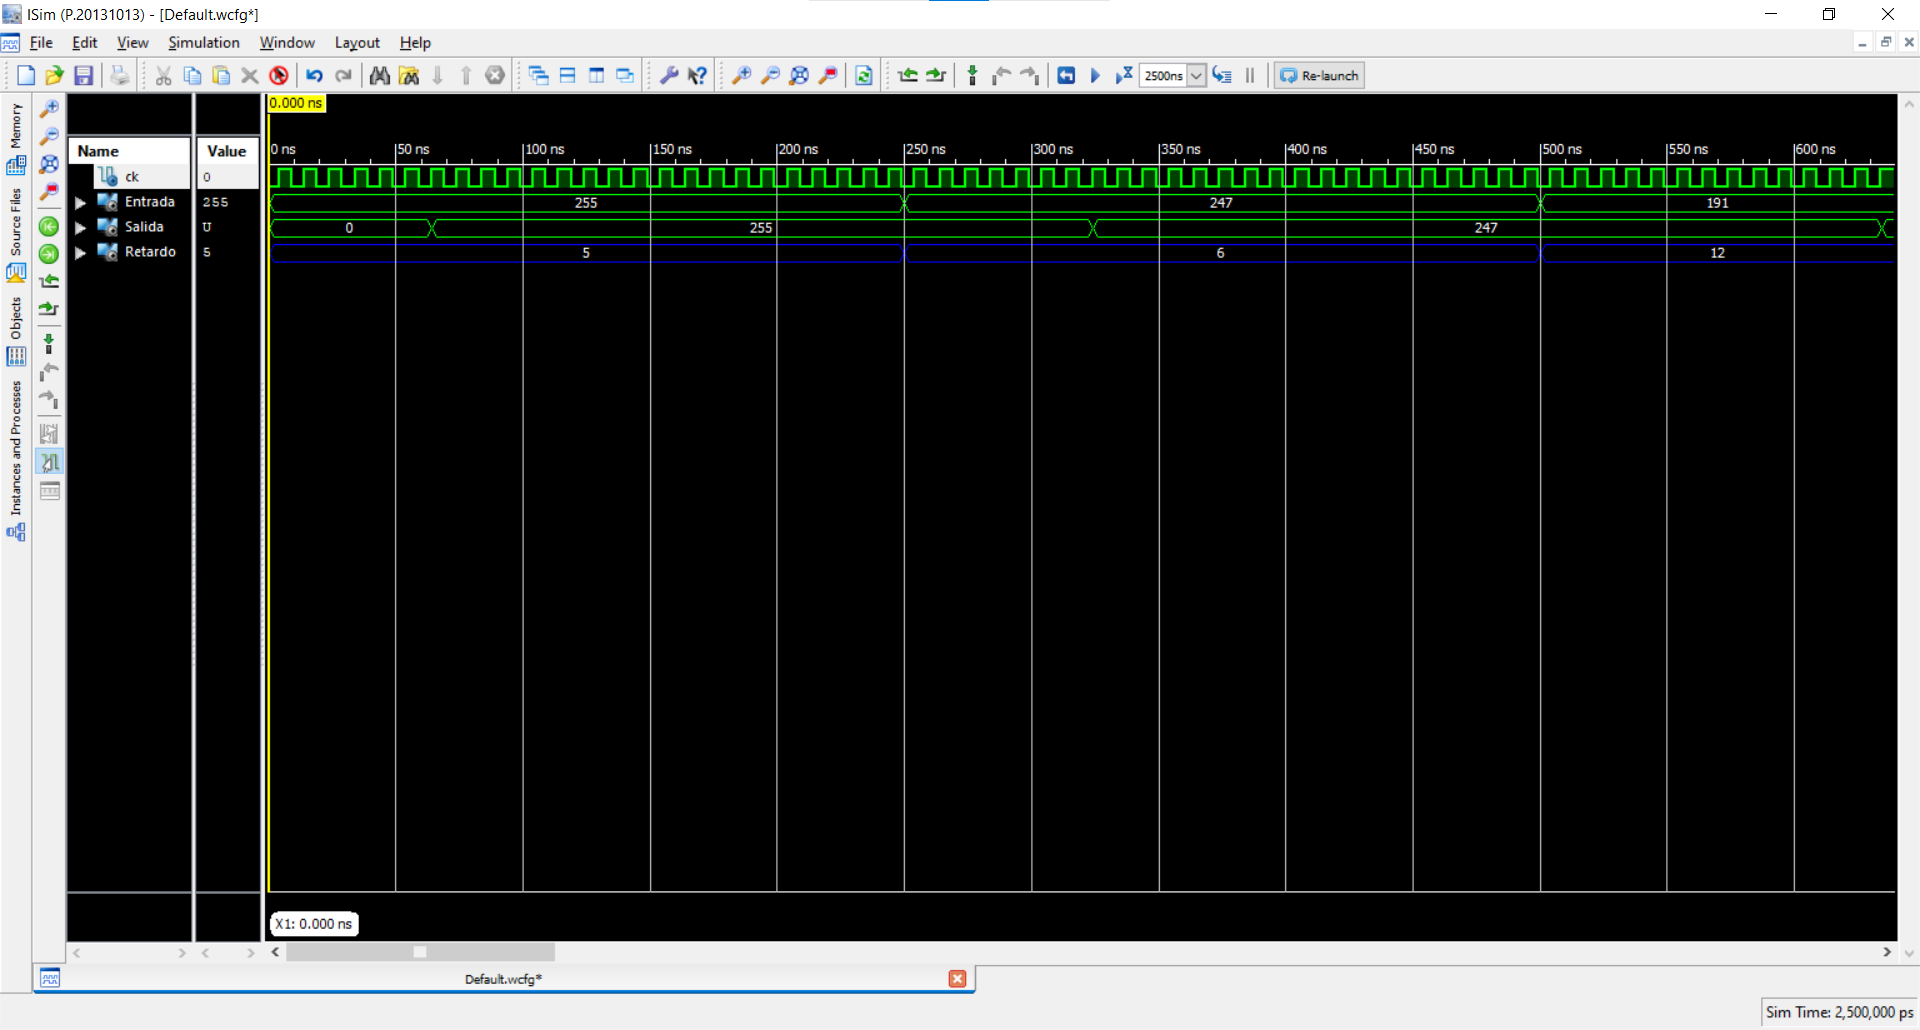
\includegraphics[scale=0.35]{images/simulacion1.png}
        \caption{Simulación realizada}
    \end{figure}
    
    \begin{figure}[H]
        \centering
        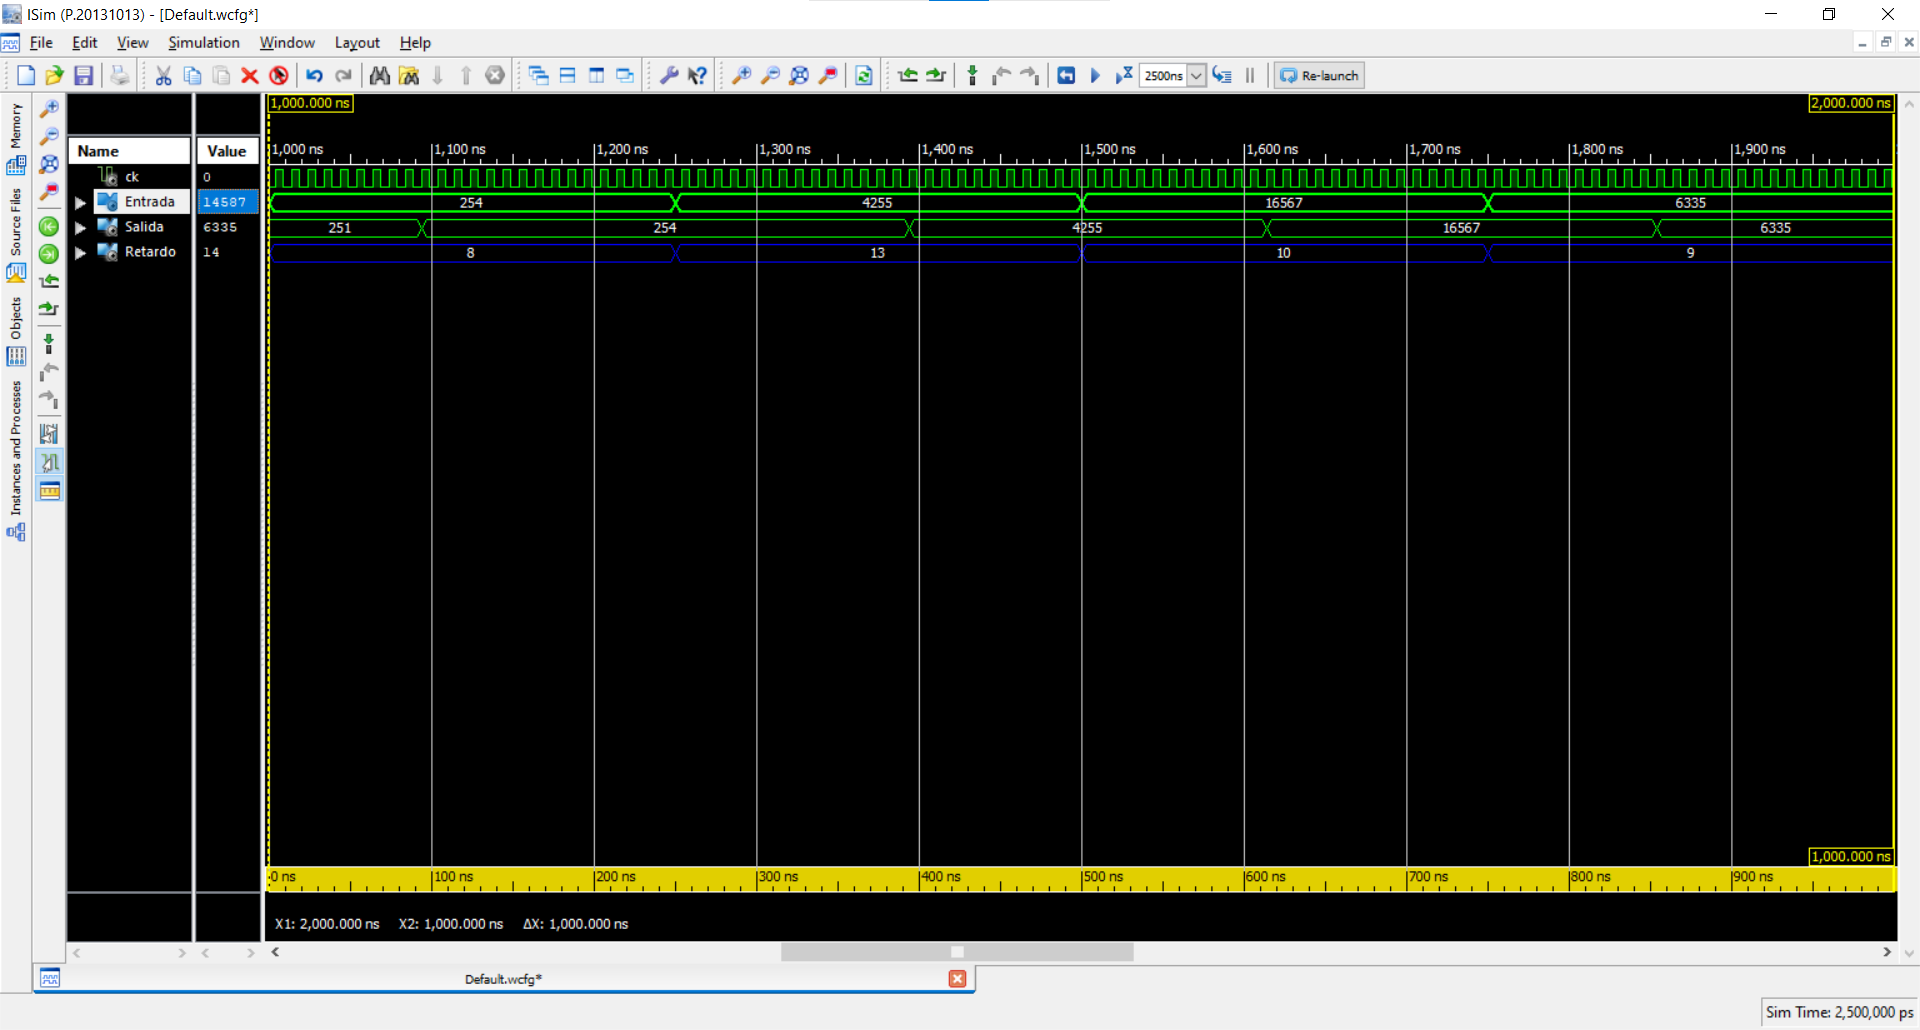
\includegraphics[scale=0.35]{images/simulacion2.png}
        \caption{Simulación realizada}
    \end{figure}
    
    \begin{figure}[H]
        \centering
        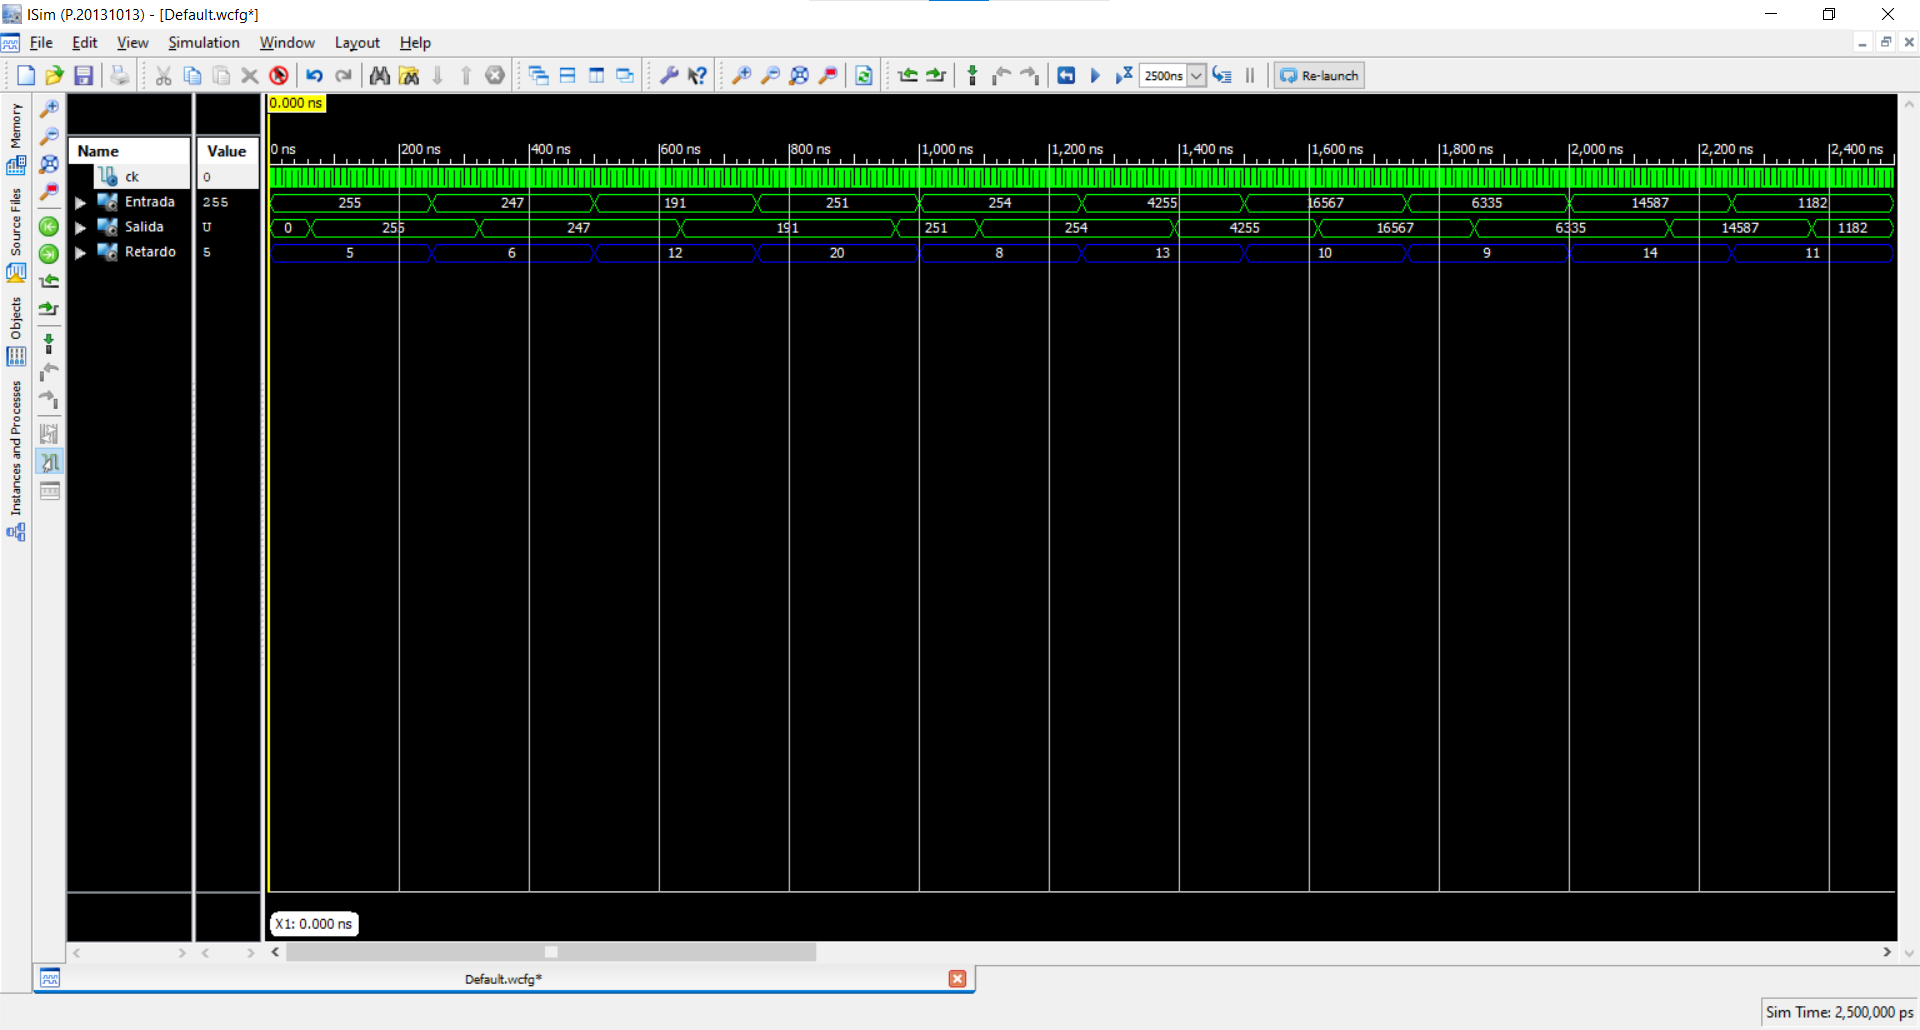
\includegraphics[scale=0.35]{images/simulacion3.png}
        \caption{Simulación realizada}
    \end{figure}
    \item Comentarios.
    
    El dispositivo simulado es un registro de desplazamiento basado en RAM, durante las distintas prácticas hemos usado varias, hechas por nosotros con flip-flops, así que el funcionamiento no es un misterio, los datos entran por D(X:0) y salen por Q(X:0), los bits se almacenan en flip-flops y estos se desplazan de un flip-flop a otro, durante un tiempo.
    
    Este dispositivo se diferencia de los usados en clase en que el retardo entre la entrada y salida es variable, modificado por la señal a(X:0), para activar esta señal he seleccionado la opción \textit{``Variable Lenght Lossless''}, esto ha modificado la latencia del dispositivo a \textit{1} ya que el último bit es registrado. El resto de parámetros no los he cambiado, excepto el \textit{width} y \textit{depth}, cuyos valores he sacado del datasheet ya que hay una tabla normalizada para la Spartan 3 y me ha parecido interesante usarlos ya que la Spartan 6 y la Spartan 3 comparten características como hemos visto en clase, \textit{width} es el tamaño de la entrada y \textit{depth} es el tamaño del retardo que podemos introducir.
    
    Posee la función de \textit{clock enable} pero no la he activado, y 3 funciones más para señalar un valor de inicio (\textit{SINIT}), hacer un clear (\textit{SCLR}) o colocar un valor (\textit{SSET}), todas estas funciones son síncronas, desactivadas porque no son parte del objetivo de la tarea.
    
    La interpretación de los datos la damos nosotros, ya que los datos que entran son los mismos que salen, pero retrasados, es decir que pueden estar en C2, en binario natural, signo-magnitud o cualquier otro formato, el diseñador es el que debe considerarlo.
    
    Es un circuito sin pipeline, pero como he comentado antes tiene latencia 1; el número de ciclos que tarda en total es la suma del número introducido en a(4:0) más 1. 
    
    Como se puede observar en la ventana de configuración no hay una sección de información como en otros dispositivos para saber la cantidad de LUTS, Slices o de recursos de la FPGA usados, dado que en el top de mi proyecto solo hay un dispositivo, he compilado el top y he mirado los recursos usados en la ventana \textit{Design Summary}.
    
    \begin{figure}[H]
        \centering
        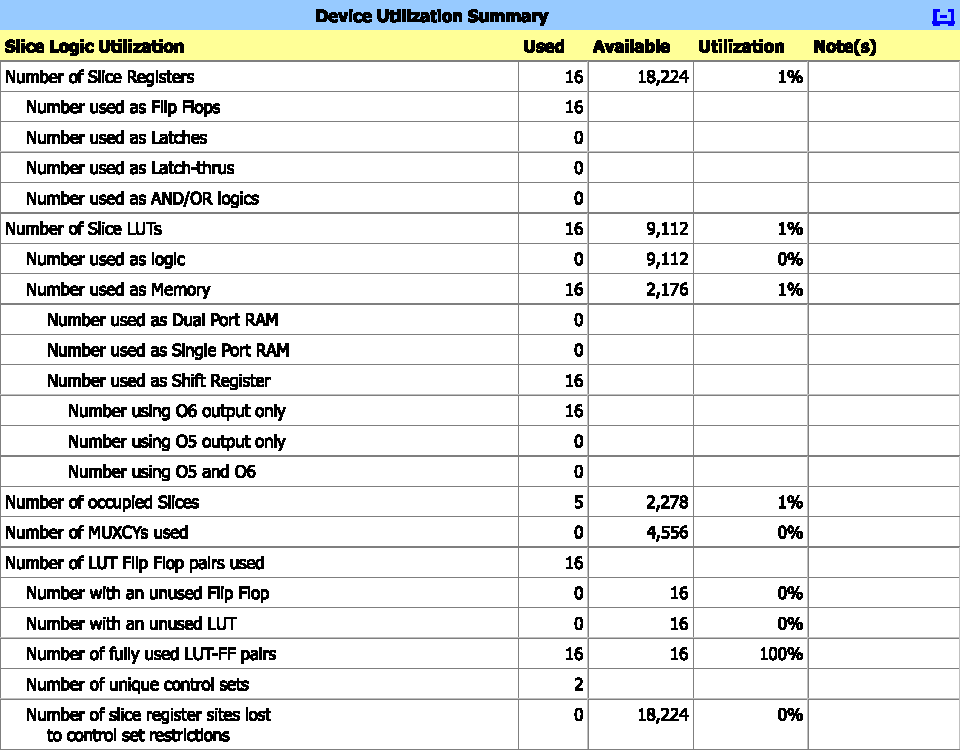
\includegraphics[scale=0.5]{images/information.pdf}
        \caption{Design Summary}
    \end{figure}
    
    Se usan 16 flip-flops, uno por cada bit de entrada, 16 Slices usados como memoria y 16 registros de desplazamiento.
    
    Respecto al código usado para la simulación he introducido los valores en las señales directamente y un retraso aleatorio mayor que 4 como se pide en la tarea; el bloque de simulación es el siguiente:
    
    \begin{figure}[H]
        \centering
        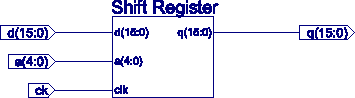
\includegraphics[scale=1]{images/registro de desplazamiento_simbolo.pdf}
        \caption{Símbolo - Registro de desplazamiento}
    \end{figure}
  
  Para la simulación he seleccionado el mayor valor de a, que en mi caso es 20, he sumado 1 y lo he multiplicado por el periodo del reloj 10ns que da como resultado 210ns, en la simulación he puesto 250ns para asegurarme de que se aprecia correctamente; en la simulación los ciclos de reloj se cuentan con el flanco de subida, para el cambio de 0 a 255 (todos los números tienen el formato unsigned decimal) hay 5 ciclos de reloj porque el retardo introducido es 4 más 1, como hemos comentado anteriormente.
    
    Como función principal tenemos el almacenamiento de datos, pero esto se puede usar de distintas forma para lograr funciones más interesantes como el almacenamiento de datos, producir retrasos e incluso hacer hacer conversiones serie/paralelo.

\end{itemize}

% \fontsize{7.5}{1.2}\selectfont
% \nocite{*}
% \bibliographystyle{IEEEtran}
% \bibliography{references}
\end{document}